%second chapter of your thesis

\chapter{Software}

\section{Arduino}

In onze code hebben we er voor geopteerd om zo veel mogelijk gebruik te maken van zelfgemaakte bibliotheken om zo de onderdelen van ons programma zo goed mogelijk van elkaar te scheiden zodat er zo weinig mogelijk verwarring mogelijk is bij het bestuderen van de code. We gebruiken dan ook slechts 1 lijn code in ons .ino bestand om een bibliotheek aan te roepen van waaruit vervolgens het hele programma wordt aangestuurd. In Figuur \ref{fig:flowchart} vindt u de flowchart van ons programma.

\begin{figure}[h]
\centering
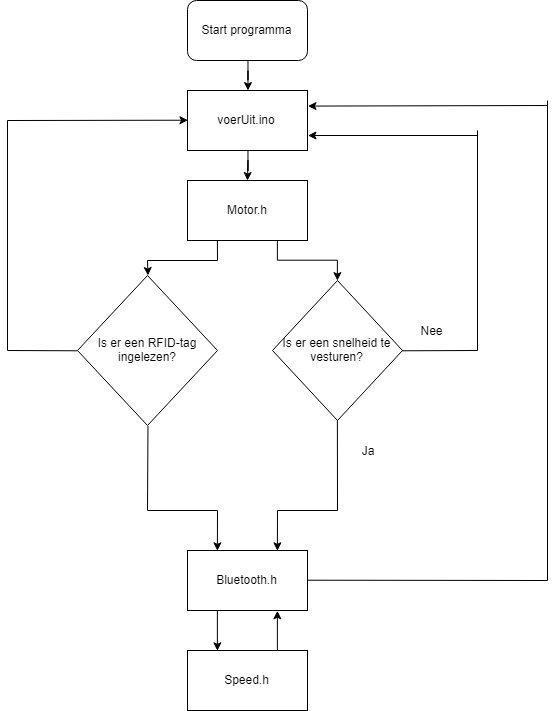
\includegraphics[width=0.5\textwidth]{flowchartLibraries.png}
\caption{Flowchart van de werking van de libraries. \label{fig:flowchart}}
\end{figure}



\subsection{Motor}

We zijn eerst en vooral begonnen met het schrijven van de Motor-bibliotheek. Deze bibliotheek wordt aangeroepen vanuit de loop van het main programma genaamd voerUit.ino. We registreren, elke keer dat de loop wordt uitgevoerd, de digitale waarden aan de sensoren en plaatsen deze voortdurend in de array van integers, genaamd LFS[ ], die vervolgens eenvoudig gebruikt kan worden voor de verwerking en generatie van de effectieve correctiewaarden. Ik stel dergelijke array voor als volgt: 000 001 waarbij nu enkel de meest rechtse infrarood sensor wit detecteert en alle 5 de andere sensoren zwart detecteren. We hebben het programma opgebouwd volgens het principe waarbij we aan de verschillende combinaties van sensoren die wit detecteren, verschillende foutwaarden associ\"eren zodat er in principe geen enkele rusttoestand is. Er wordt als het ware voortdurend gecorrigeerd maar in zo een kleine mate dat dit amper zichtbaar is voor ons. In ons programma krijgt de kleinste fout, namelijk de buitenste sensor die wit detecteert, de foutwaarde 1.1. In het allerslechtste geval, namelijk 000 100, waarbij een van de middelste sensoren wit detecteert, krijgt deze situatie een foutwaarde van 4.6 mee. Deze error values worden elke keer dat het programma doorlopen wordt, aangepast indien de toestand van \'e\'en van de sensoren gewijzigd werd. Deze waarden zijn niet zomaar gekozen maar we hebben uitgezocht welke combinatie van PD-constanten en error values tot de beste prestaties kon leiden. Een voorbeeld van dergelijke code vindt u in Listing \ref{listing:detectiealgoritme}. De error value die gegenereerd werd, wordt vervolgens gebruikt in de corrigeer-methode waarin de werking van ons PD-algoritme in verwerkt zit.

\lstinputlisting[basicstyle=\tiny ]{detectiealgoritme.txt}
\begin{lstlisting}[caption={Het algoritme die de foutwaarden toekent aan de verschillende situaties} \label{listing:detectiealgoritme}]
\end{lstlisting}

\subsection{PD-algoritme}

Dit algoritme is vrij beknopt maar toch zeer interessant aangezien het de prestaties van het wagentje heel erg verbetert. PID is de afkorting voor Proportioneel, Integrerend en Differenti\"erend. Deze regelaar is dus in staat om verschillende soorten fouten te detecteren en in de juiste mate te reageren om zo oscillaties weg te werken en een stabiel voertuig te verkrijgen. Het proportioneel aandeel in de regelaar is een vermenigvuldiging van KP met het verschil van de waarde die je zou willen dat de sensoren meten, verminderd met de waarde die effectief geregistreerd wordt. De integrerende actie zorgt voor een foutcorrectie die ontstaat door het constant optellen van de fout. Hoe langer een fout zich dus voordoet, des te groter de waarde van de integrerende term zal zijn. Ook deze waarde wordt nog vermenigvuldigd met een constante namelijk KI. Als laatste hebben we nog de differenti\"erende term. Deze term is functie van de snelheid van verandering van de fout. Wanneer de afwijking tussen de gewenste waarde en de gemeten waarde toeneemt, zal de D-term in functie van de snelheid van verandering reageren om zo een mogelijks zeer groot wordende fout te beperken in grootte. Ook in de andere richting zal de correctie afgeremd worden wanneer de gemeten waarde nadert naar de gewenste waarde. 

De P-waarde wordt gelijkgesteld aan de error value die we hierboven ge\"introduceerd hebben. De I-waarde hebben we in dit project niet gebruikt aangezien deze waarde enorm snel toeneemt en niet eenvoudig was om perfect in te stellen. Achteraf gezien bleek deze term niet noodzakelijk om een stabiel rijdende robot te verkrijgen. We maken dus gebruik van een PD-regelaar niet van een PID-regelaar. De D-waarde wordt slechts om de 500 milliseconden vervangen door een nieuwe waarde. Mochten we deze tijdsrestrictie niet verwerkt hebben in de code, dan zou de D-waarde amper invloed hebben aangezien ons programma meer dan 1000 keer per seconde wordt uitgevoerd en dus met andere woorden, wanneer de fout gedetecteerd wordt en de D-waarde zijn correctie wilt uitvoeren, er onmiddellijk een nieuwe waarde wordt geregistreerd die meestal opnieuw diezelfde waarde is waardoor de D-correctiewaarde wegvalt. We testten de snelheid van ons programma uit met behulp van onderstaande code om tot dergelijk inzicht te komen en verkregen een uitvoer in de Seri\"ele monitor van 0 milliseconden wat dus illustreert dat het programma meer dan 1000 keer per seconde wordt uitgevoerd.

\lstinputlisting[basicstyle=\tiny ]{tijdsmeting.txt}
\begin{lstlisting}[caption={Het algoritme om de frequentie van de uitvoering van het programma te bepalen} \label{listing:tijdsmeting}]
\end{lstlisting}

De D-waarde en de P-waarde worden vervolgens nog vermenigvuldigd met de KP en KD constanten, zoals te zien in Listing \ref{listing:PID},  die we met behulp van beproeving hebben bepaald om de beste prestaties te verkrijgen. De som van deze producten wordt opgeslagen in PIDvalue en wordt meegegeven in de rij-methode. Wat niets anders is dan een methode voor het instellen van de algemene snelheid en de snelheid per wiel, rekening houdend met de PIDvalue die we net definieerden. 

\lstinputlisting[basicstyle=\tiny ]{PID.txt}
\begin{lstlisting}[caption={Het PD-algoritme dat wij hanteren} \label{listing:PID}]
\end{lstlisting}


\subsection{Detectie-algoritme}

Een extra functionaliteit die we verwerkt hebben in onze code die van belang is bij de error value, is het feit dat als alle sensoren zwart detecteren dat de robot weet of hij zich nu binnen of buiten het parcours bevindt waardoor zijn error values verschillen. Bij alle verschillende situaties waarin de sensoren zich kunnen bevinden, wordt er een boolean aangepast. Zo zal de boolean limitReached in alle gevallen false zijn behalve in de 2 gevallen 000 100 en 001 000, dan zal de boolean true gemaakt worden. Dit zijn de situaties waarbij de robot over de buitenlijn aan het gaan is en de ene arm zich buiten het parcours bevindt en de andere arm zich binnen bevindt. Indien de fout nog een klein beetje verder toeneemt verkrijg je de situatie 000 000 waarbij de witte lijn zich tussen de sensoren bevindt. De robot zal nu zeer hevig gaan corrigeren aangezien de boolean limitReached true is. 

Wanneer we werken met 2 armen ontstaan er extra problemen, namelijk naar welke arm moet er geluisterd worden en in welke richting moet de robot uitwijken wanneer alle sensoren zwart zijn. Elke keer dat er een arm wit registreert, wordt de boolean rechtersensorActief aangepast naar true of false naargelang de arm die het wit detecteert. Wanneer de sensoren volgende situatie registreren 000 001, dan wordt de boolean rechtersensorActief op true gezet. Wanneer je in dit geval los komt van de lijn, weet het programma dat het naar rechts moet gaan corrigeren om de rechterlijn terug te intercepten. Maar wanneer de boolean limitReached op true staat, wilt dat zeggen dat de situatie 000 100 zich net voordien heeft voorgedaan en het wagentje zich dus eigenlijk te ver rechts van het circuit bevindt. Nu zal het wagentje naar links moeten corrigeren met een grotere factor dan normaal aangezien de boolean limitReached deze hevige reactie genereert.


De 2e functionaliteit dat we hebben toegevoegd is het principe dat de robot weet of hij zich links of rechts van de lijn bevindt en zo dus in de juiste richting kan corrigeren. Dit was nodig om de 2 armen te kunnen laten samenwerken.


\subsection {Communicatie}

In de methode bepaalPID() bevinden er zich nog 2 andere methodes die aangeroepen worden, namelijk verstuurSnelheid() en verstuurTag(). Beide methodes bevatten een methode die de communicatie met de Bluetooth-bibliotheek afhandelt. In verstuurSnelheid() bevindt zich de methode bluetooth.stuurSnelheid(). In de Bluetooth-bibliotheek wordt er vervolgens een waarde opgevraagd van de Speed-bibliotheek waarin zich het algoritme voor de registratie van de huidige snelheid van de robot bevindt die je vindt in Listing \ref{listing:snelheidsregistratie}. De snelheidswaarde wordt telkens wanneer het wieltje een rotatie maakt aangepast met behulp van een eenvoudige snelheidsvergelijking. De snelheid wordt vervolgens 1 keer per seconde gereturned naar de Bluetooth-bibliotheek van waar het met behulp van Software Serial verstuurd wordt met de HC-05 naar de Raspberry Pi. 

\lstinputlisting[basicstyle=\tiny ]{snelheidsregistratie.txt}
\begin{lstlisting}[caption={Methode om de snelheid te registreren} \label{listing:snelheidsregistratie}]
\end{lstlisting}

De verstuurTag()-methode is een methode die instaat voor het correct versturen van de RFID-ID van de tags die zich onder de mat bevinden. We stootten daarbij op het probleem dat de mfrc522 gebruikt maakt van de SPI-pinnen. Deze pinnen waren echter reeds in gebruik door de motoraansturing die verwerkt is in onze printplaat en volledig geroute was. De RFID-lezer anders aansluiten was geen optie alsook de printplaat opnieuw routen zagen we niet onmiddellijk zitten. We hebben vervolgens geopteerd om een hulp-arduino te maken die vervolgens zou instaan voor het lezen van de RFID-tags en deze informatie vervolgens via UART, met behulp van de TX-pin, te verzenden naar de RX-pin van de hoofd-Arduino. Hierdoor hebben we het probleem van de SPI-pinnen kunnen oplossen en hebben we via een eenvoudig protocol, communicatie tot stand gebracht tussen beide Arduino's. De ID-waarde die de hoofd-Arduino vervolgens ontvangt, wordt naar de Bluetooth-bibliotheek geleid vanwaar het via Bluetooth verzonden wordt naar de Raspberry Pi.

\lstinputlisting[basicstyle=\tiny ]{communicatie.txt}
\begin{lstlisting}[caption={Algoritme voor het versturen van data via de HC-05 naar de Raspberry Pi} \label{listing:communicatie}]
\end{lstlisting}

\section{Raspberry Pi}


Om de Raspberry Pi werkende te krijgen, hebben we eerst enkele packages moeten installeren om het mogelijk te maken een seri\"ele Bluetooth communicatie tot stand te brengen. Eerst en vooral installeerden we een Bluetooth Interface met behulp van onderstaand commando.

\lstinputlisting[ ]{installbluetooth.txt}
\begin{lstlisting}[ ]
\end{lstlisting}

We kunnen nu via preferences onze bluetooth apparaten beheren en pairen met de HC-05 van onze Arduino. Van zodra we verbonden zijn, komt er een melding dat we gebruik maken van rfcomm0. Deze naam hebben we ook nodig om ons Python programma te laten samenwerken met de Bluetoothchip op de Raspberry Pi. 

Het Python programma is bij ons vrij beknopt. Het is een programma dat voortdurend luistert of er data binnenkomt via Bluetooth en indien er data binnenkomt, deze data vervolgens onmiddellijk afprint. De 2 enige momenten waarbij de Raspberry Pi dus data ontvangt is de snelheid die elke seconde doorgestuurd wordt en elke keer er over een RFID-tag gereden wordt waarbij de ID doorgestuurd wordt. Het Python programma waarvan wij gebruik gemaakt hebben vindt u in Listing \ref{listing:raspberrypicode}

\lstinputlisting[basicstyle=\tiny ]{raspberrypicode.txt}

\begin{lstlisting}[caption={Code die wordt uitgevoerd door de Raspberry Pi} \label{listing:raspberrypicode}]
\end{lstlisting}



